
\begin{thm}[Pascal's Formula]\index{Pascal's Formula}
    Given positive integers \(0<k<n\), 
    \begin{equation}\label{eq:pascal}
        \binom{n+1}{k+1}=\binom{n}{k}+\binom{n}{k+1}.
    \end{equation}
\end{thm}

\begin{exposition}[Pascal's Triangle]\index{Pascal's Triangle}
    Using Pascal's Formula (equation \ref{eq:pascal}) we can create Pascal's Arithmetic Triangle:
    \begin{figure}[H]
        \centering
        % \inputtikz{pascals_triangle}
        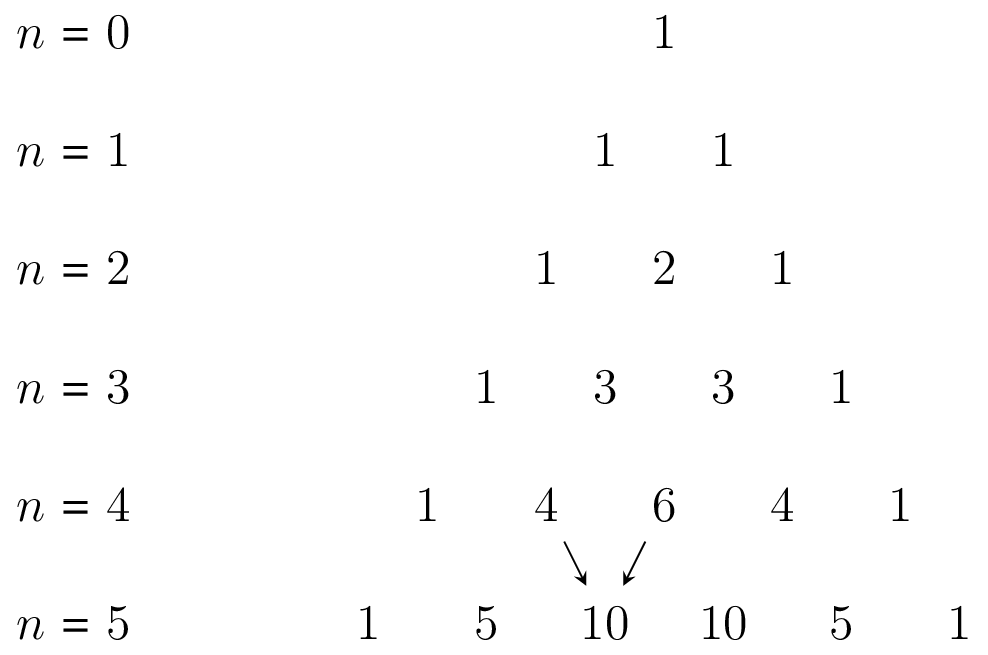
\includegraphics[scale=0.24,alt={the first six rows of pascal's triangle}]{images/created/pascals_triangle.png}
        \caption{Pascal's Triangle}
        \label{fig:pascal-tirangle}
    \end{figure}
    which lists the \emph{binomial coefficients} for each value of \(n\).
\end{exposition}

\begin{thm}[Binomial Theorem]\index{binomial theorem}
    Given a positive integer \(n\) and variables \(a\) and \(b\):
    \begin{align}\label{eq:binom}
        (a+b)^n&=(a+b)(a+b)\cdots(a+b)\\
            &=a^n+\binom{n}{1}a^{n-1}b+\binom{n}{2}a^{n-2}b^2+\cdots+\binom{n}{n-1}ab^{n-1}+b^n\\
            &=\sum_{k=0}^{n}\binom{n}{k}a^{n-k}b^k
    \end{align}
\end{thm}

\begin{practiceprob}[Sum of Pascal Rows]
    Show that the sum of the coefficients in row \(n\) of Pascal's Triangle is \(2^n\).  (Hint: \((1+1)=2\))
    \vspace{0.25\textheight}
\end{practiceprob}
